\documentclass{article}
\usepackage{graphicx}
\topmargin  0.0in
\headheight  0.15in
\headsep  0.15in
\footskip  0.2in
\textheight 8.45in

\oddsidemargin 0.56in
\evensidemargin \oddsidemargin
\textwidth 5.8in

\usepackage{clrscode}
\input{epsf}

\pagestyle{myheadings}
\markright{\bf Volume Grid Format}

\begin{document}

\title{The Volume Grid (vog) File Format}

\author{ Edward Luke \\
\it luke@cse.msstate.edu}


\maketitle

% example of figure including code
%\begin{figure}[htbp]
%  \centerline{ \epsfxsize=5.5in \epsfbox{figures/constructs.eps}}
% \caption{Four Basic Container Categories}
% \label{constructs}
%\end{figure}

\section{Introduction}

The volume grid file format is a format implemented using the HDF5
library.  The contents of the file include the following top level
groups: {\tt file\_info}, {\tt node\_info}, {\tt surface\_info}, and
{\tt face\_info}.

\subsection{\tt file\_info}

The {\tt file\_info} group contains general information about the mesh.  This
includes the following attributes:
\begin{enumerate}
  \item {\tt numCells} : integer describing the number of cells in the mesh.
  \item {\tt numFaces} : integer describing the number of faces in the mesh.
  \item {\tt numNodes} : integer describing the number of nodes in the mesh.
\end{enumerate}

\subsection{\tt node\_info}

The {node\_info} group contains an array of 3-D vectors in a dataset
under the name {\tt positions}.  This array has a length equal to the
{\tt numNodes} attribute given in the {\tt file\_info} group.


\subsection{\tt surface\_info}

The {\tt surface\_info} group contains boundary condition information.
For each named boundary condition this group contains a group with the
name of the boundary surface. Under this group is an attribute {\tt
  Ident} that contains the integer tag associated with this boundary.
This tag will be how the boundary faces are identified in the {\tt
  face\_info}

\subsection{\tt face\_info}.

The {\tt face\_info} group contains a compressed data structure that
identifies the nodes and cells associated with each face.  The
compression factor this data structure provides depends on the
locality of the data within the mesh.  Usually cells are ordered using
a space filling curve to improve compression as well as to help
improve performance of parallel file processing.  The node and face
orderings are also optimized to improve locality and increase
compression of these data structures.  In this data structure faces
are written out in small clusters of variable size.  The {\tt
  cluster\_sizes} data set is an array of the size in bytes of each
cluster, while the attribute {\tt cluster\_info} dataset is a
concatenation of all face clusters.

The face clusters store, in a compressed form, the nodes that form a
face and the cells that lie on the left and right sides of the face.
These relationships are identified as {\tt face2node} that lists the
nodes that form the face in an ordering that defines a normal vector
that points out of the left cell and into the right cell.  The cells
on either side of a face are defined by {\tt cl} (cell left) and {\tt
  cr} (cell right) according to the right hand rule as illustrated in
figure \ref{fig:face}.  Cells are numbered starting from $0$ while
negative cell numbers are reserved for marking boundary surface facets
with a surface identifier.  All boundary faces are oriented so that
the normal points out of the domain such that {\tt cr} right cell will
contain a negative of the boundary surface id associated with that
boundary face.  Finally for all interior faces (faces in which {\tt
  cl} and {\tt cr} are positive numbers) the face must be oriented
such that there exists some unique coloring that can be applied to the
cells where the left cell has a lower color than the right cell.  In
other words, the faces are oriented such that one cannot follow faces
from left to right and ever arrive back to the same cell from which
they started.  This coloring is used when the symmetric Gauss Seidel
solver is employed and is usually determined by the level parameter
that is obtained from a depth first search of cell-to-cell
connectivities implied by the faces.

\begin{figure}[htbp]
\begin{center}
  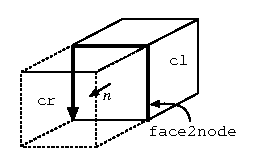
\includegraphics[width=10cm]{face}
 \caption{The {\tt face2node} map and its relationship to neighboring cells}
 \label{fig:face}
\end{center}
\end{figure}

\end{document}
